\chapter{Návrh funkcionality}
	V tejto kapitole opíšeme, ako je naše riešenie navrhnuté. Vysvetlíme, ako budeme postupovať v prípade nahrávania, sťahovania, zdieľania a čo spravíme, keď už nechceme zdieľať dáta. Na záver kapitoly uvedieme, aký môže mať toto riešenie problém a ako by sme ho vedeli riešiť.
	
	\section{Prerekvizity}
	
		Aby naše riešenie fungovalo, budeme potrebovať server, ktorý bude poskytovať API na komunikáciu s databázou a bude hostovať naše webové rozhranie, databázu, kam budeme ukladať používateľove kľúče a kľúče k súborom, a cloudové úložisko, ktoré bude zabezpečovať prácu so súbormi. Cloud musí poskytovať rozhranie, pomocou ktorého vieme nahrávať a sťahovať dáta a musí byť schopný autorizovať rôznych používateľov pre prístup k dátam iných používateľov. Vďaka tomu budeme môcť zdieľať súbory. 
		
	\section{Registrácia}
		
		Keď sa používateľ rozhodne používať našu službu, musí sa nejakým spôsobom identifikovať a autentifikovať. Identifikácia vyžaduje, aby si každý používateľ zvolil meno a aby sme ho mohli autentifikovať potrebuje heslo. Druhou možnosťou je využiť tretiu službu ako napríklad cloud, kde budeme ukladať súbory. Toto je možné napríklad pomocou protokolov oAuth alebo openID. Nech už vyberieme jeden alebo druhý spôsob, budeme jednoznačne vedieť s kým komunikujeme. S touto informáciou vyzveme používateľa, aby si zvolil svoje univerzálne heslo, pomocou ktorého bude autorizovať akcie ako nahrávanie, sťahovanie, zdieľanie a zrušenie zdieľania dát.
		
		Následne v používateľovom prehliadači vygenerujeme verejný a privátny kľúč, ktorý symetricky zašifrujeme pomocou už zvoleného univerzálneho hesla. Verejný aj zašifrovaný privátny kľúč uložíme na serveri, kde budú mať všetci používatelia prístup k verejným kľúčom, no k privátnym len jeho vlastníci. Vďaka tomu, že privátny kľúč je zašifrovaný, server nemá žiadnu informáciu o privátnom kľúči a teda schéma ostane bezpečná. 
		
		Ďaľšou možnosťou bolo uložiť privátny kľúč na užívateľovom počítači. Toto sme sa rozhodli nevyužiť z dôvodu náročného manažmentu kľúčov na rôznych zariadeniach. Napríklad pri strate zariadenia by to vyžadovalo zmenu privátneho kľúča, čo by implikovalo nutnosť prešifrovania všetkých súborových kľúčov. Distribúcia kľúča do rôznych zariadení by bola v rukách používateľa, čo by mohlo byť nepohodlné.
		
		
		\begin{figure}[H]
			\begin{center}
				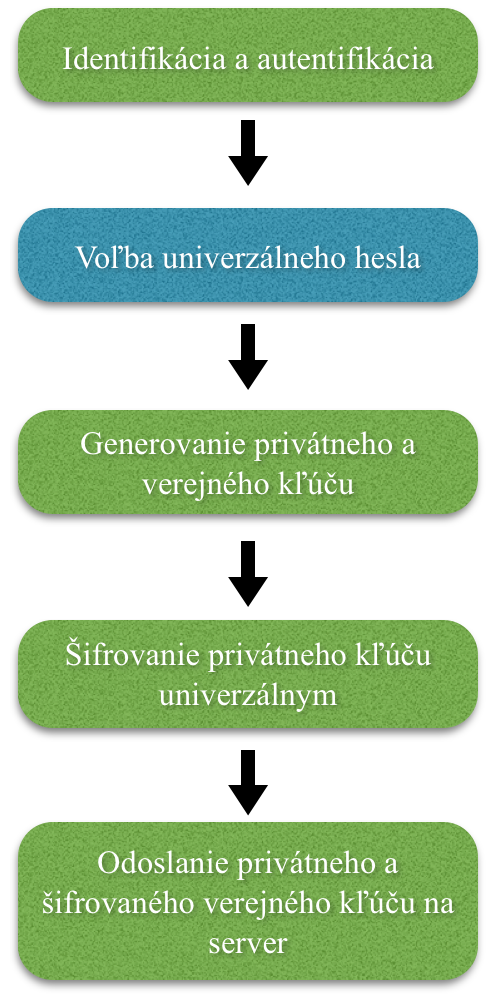
\includegraphics[width=0.5\linewidth]{images/registracia.png}
				\caption{Navrhovaný priebeh registrácie v systéme SecureCloud}
			\end{center}
		\end{figure}
	
	\section{Nahrávanie dát}
	
		Používateľ sa autentifikuje a v prehliadači sa pomocou pseudonáhodného generátora vygeneruje náhodný kľúč. Ten využije na zašifrovanie súboru a vypýta si od servera svoj verejný kľúč. Pomocou verejného kľúča zašifruje heslo k súboru a v takomto tvare ho už môže poslať na server. Keďže heslo je zašifrované a server nemá žiadnu informáciu o privátnom kľúči, nevie získať dáta v otvorenom tvare. Následne už len stačí zašifrovaný súbor nahrať na cloudové úložisko.
		
		\begin{figure}[H]
			\begin{center}
				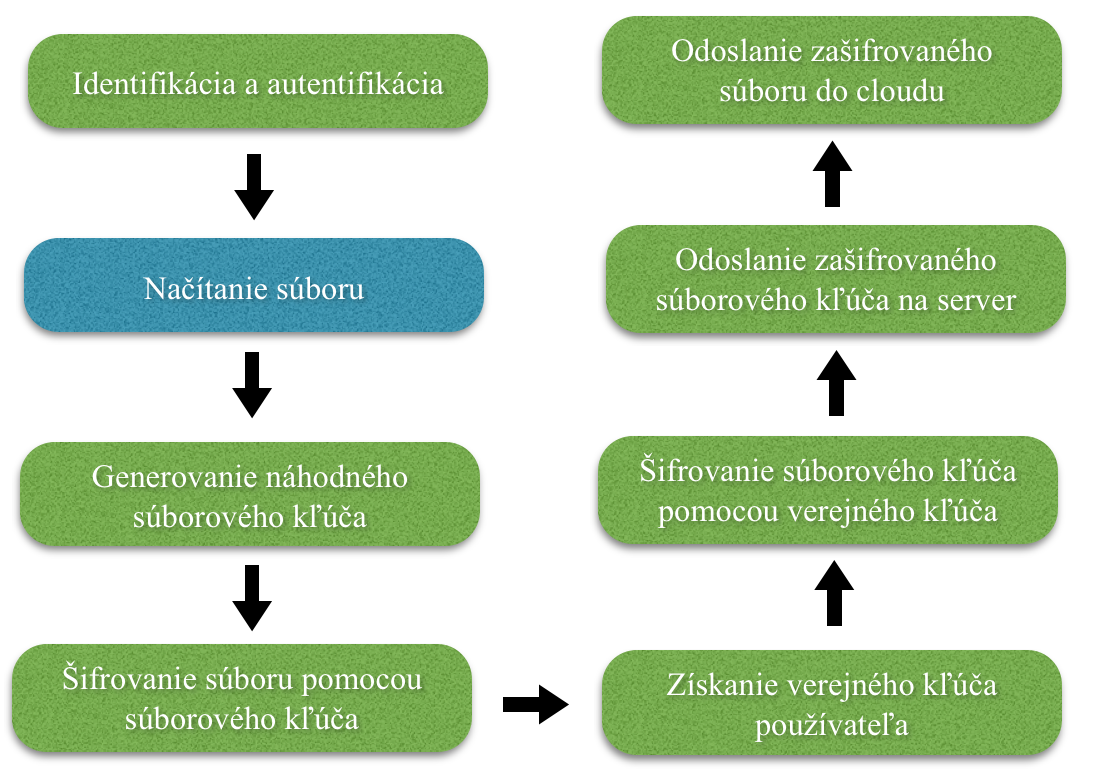
\includegraphics[width=1\linewidth]{images/nahravanie.png}
				\caption{Nahrávanie dát}
			\end{center}
		\end{figure}
				
	\section{Sťahovanie dát}
	
		V prípade, že privátny kľúč je uložený na serveri, vypýtame si ho a požiadame používateľa o jeho univerzálne heslo, aby sme mohli privátny kľúč dešifrovať. S privátnym kľúčom môžeme následne dešifrovať heslo k súboru, ktoré si opäť vypýtame od servera. V tejto chvíli máme k dispozícii kľúč k súboru a teda nám stačí stiahnuť súbor z cloudu a rozšifrovať ho pomocou zmieneného kľúča. 
		
		\begin{figure}[H]
			\begin{center}
				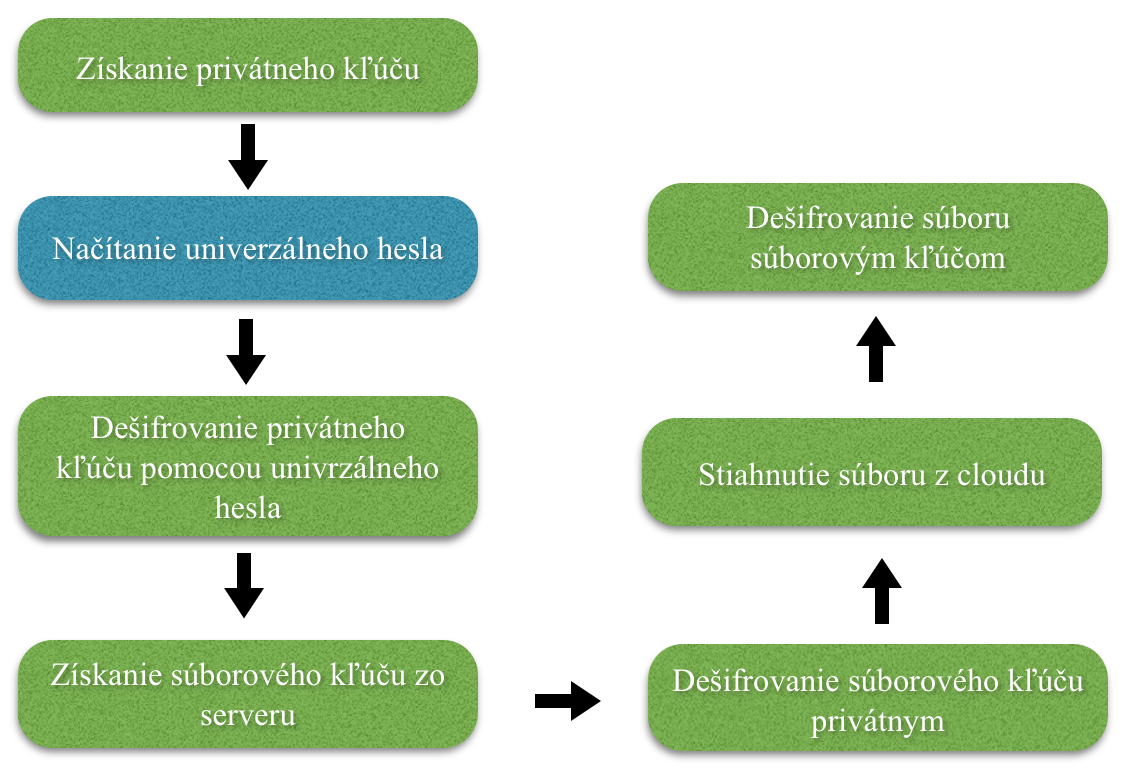
\includegraphics[width=1\linewidth]{images/stahovanie.png}
				\caption{Sťahovanie dát}
			\end{center}
		\end{figure}	
		
	\section{Zdieľanie}
	
		Chceme zdieľať súbor, ktorý je uložený v zašifrovanej forme na cloude. Na zdieľanie je nutné, aby cieľový príjmateľ bol zaregistrovaný na našom serveri a mal vygenerovaný privátny a verejný kľúč. Zdieľanie bude prebiehať tak, že používateľ si od servera vypýta privátny kľúč, ktorý dešifruje pomocou svojho univerzálneho kľúča. Následne požiada server o zašifrovaný kľúč k súboru, ktorý dešifruje pomocou privátneho kľúča. Dešifrovaný kľúč k súboru potom zašifruje verejným kľúčom používateľa, s ktorým chce dáta zdieľať a takýto kľúč k súboru uloží na serveri. Následne pošle požiadavku na cloud, aby povolil prístup k súboru nášmu adresátovi. Ten má potom prístup ku kľúču na dešifrovanie súboru a tiež si môže stiahnuť zašifrovaný súbor z cloudu.
		
		\begin{figure}[H]
			\begin{center}
				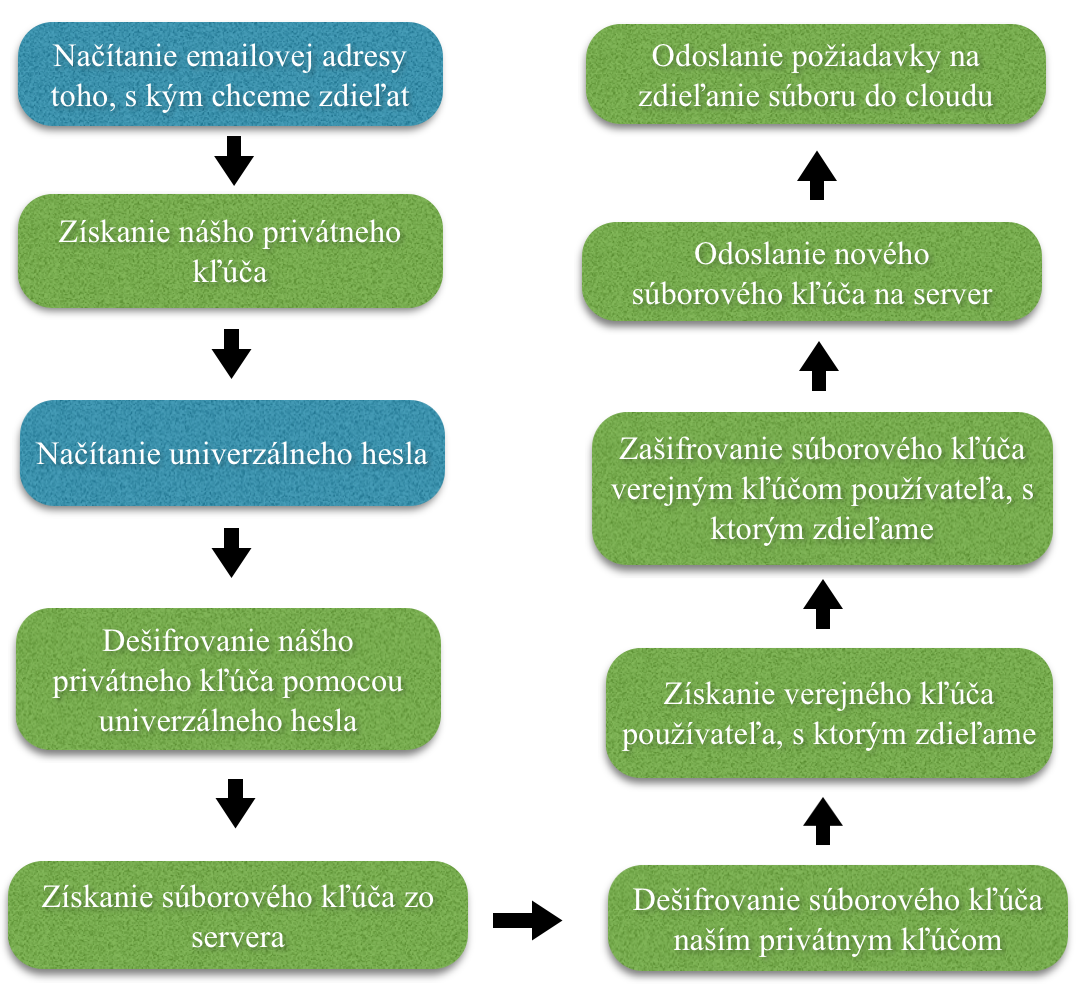
\includegraphics[width=1\linewidth]{images/zdielanie.png}
				\caption{Zdieľanie dát}
			\end{center}
		\end{figure}
		
	\section{Zrušenie zdieľania}
	
		Keď sa rozhodneme zrušiť zdieľanie súboru, stačí, aby sme požiadali cloudové úložisko o revokovanie prístupu k súborom. Keby sa používateľ, s ktorým ten súbor zdieľame, rozhodol zverejniť ho alebo inak distribuovať, šifrovanie nám nepomôže, pretože už si mohol spraviť kópiu nešifrovanej verzie. Preto stačí revokovať prístup na cloude a nemusíme súbor prešifrovať. V prípade, že sa súbor zmení a budeme ho znova uploadovať, prebehne opäť procedúra ako pri nahrávaní dát. Nové informácie teda nebudú kompromitované.
		
		
	\section{Bezpečnostný problém}
	
		V prípade, že by sa poskytovateľ cloudového úložiska a server rozhodli ukradnúť používateľove dáta, nastane problém. Predstavme si teda nasledujúcu situáciu. Používateľ chce zdieľať súbor, poprosí server o súborový kľúč, ktorý dešifruje. Vypýta si od serveru verejný kľúč používateľa, s ktorým chce zdieľať, zašifruje ním súborový kľúč a pošle ho na server. V tejto chvíli sa mohlo stať, že server odoslal verejný kľúč, ku ktorému vlastní privátny kľúč. Ak sa mu podarilo dohodnúť s poskytovateľom cloudového úložiska, tak v tejto chvíli vedia dešifrovať súbor. Cloud poskytne súbor a server poskytne kľúč k dešifrovaniu.
		
		\subsubsection{Riešenie}
		
		Ako čiastočné riešenie problému by sme mohli navrhnúť podpisovanie verejného kľúča. Čiastočným preto, lebo aj tu musíme byť schopní overiť, komu patrí verejný kľúč. Týmto by sme do problému zahrnuli ďalšiu stranu, ktorou by mohla byť certifikačná autorita, čo by mohlo znížiť pravdepodobnosť hrozby. No v našom riešení toto vynecháme.
		
		
		